\documentclass[preprint,12pt,3p,nopreprintline]{elsarticle}

% ============================================================
% Encoding and general packages
% ============================================================

\usepackage[utf8]{inputenc}
\usepackage[T1]{fontenc}

\usepackage{fancyhdr}
\usepackage{pdfpages}
\usepackage{mdwlist}
\usepackage{bm}
\usepackage{blindtext}
\usepackage{array}
\usepackage{multicol}
\usepackage{multirow}
\usepackage{enumitem}

% natbib is already supported by elsarticle
\usepackage{natbib}

\usepackage{url}
\usepackage{graphicx}
\usepackage{caption}

\usepackage{amsmath}
\usepackage{amsthm}
\usepackage{amsfonts}
\usepackage{mathrsfs}
\usepackage{amssymb}

\usepackage{mdframed}
\usepackage{xcolor}
\usepackage{fourier-orns}
\usepackage{geometry}
\usepackage{parskip}
\usepackage{listings}
\usepackage{setspace}

\usepackage{imakeidx}
\usepackage{etoolbox}

\usepackage{booktabs}
\usepackage{dcolumn}
\usepackage{adjustbox}
\usepackage{subfig}
\usepackage{lscape}
\usepackage{float}
\usepackage{empheq}
\usepackage{tabularx}

% Force floats on float-only pages to start at the top
\makeatletter
\setlength{\@fptop}{0pt}
\makeatother

% ============================================================
% Hyperlinks
% ============================================================

\usepackage[
    plainpages=false,
    pdfpagelabels,
    pagebackref=false,
    hyperindex,
    breaklinks=true,
    colorlinks=true,
    citecolor=black,
    linkcolor=black,
    urlcolor=black,
    filecolor=black,
    bookmarksopen=true
]{hyperref}

\pdfstringdefDisableCommands{%
  \def\corref#1{}%
  \def\fnref#1{}%
}
% ============================================================
% Bibliography
% ============================================================

\biboptions{numbers,sort&compress}

% ============================================================
% Listings
% ============================================================

\lstset{
    language=Python,
    basicstyle=\fontsize{10}{12}\selectfont\ttfamily,
    keywordstyle=\color{blue},
    commentstyle=\color{green!60!black},
    stringstyle=\color{red},
    showstringspaces=false,
    breaklines=true,
    frame=single,
    numbers=left,
    numberstyle=\tiny\color{gray},
    captionpos=b,
    escapeinside={(*@}{@*)}
}

% ============================================================
% General mathematical definitions
% ============================================================

\DeclareMathOperator{\sech}{sech}

\newcommand{\sen}{\mathrm{sen}}
\newcommand{\dd}{\mathrm{d}}

\newcommand{\keywords}[1]{%
    \textbf{\textit{keywords:}} #1%
}

\newcommand{\palavraschave}[1]{%
    \textbf{\textit{palavras-chave:}} #1%
}

\newcommand{\EE}{\mathbf{e}}
\newcommand{\RR}{\mathrm{R}}
\newcommand{\GG}{\mathbf{G}}
\newcommand{\TT}{\mathrm{T}}

% ============================================================
% Geometry notation for this paper
% ============================================================

% Point
\newcommand{\pt}[1]{\mathbf{#1}}

% Segment
\newcommand{\seg}[1]{\mathbf{#1}}

% Positive segment length
\newcommand{\seglen}[1]{\lvert\mathbf{#1}\rvert}

% Directed segment
\newcommand{\dseg}[1]{\overline{\mathbf{#1}}}

% Power of a point
\DeclareMathOperator{\Pot}{Pot}

% ============================================================
% Equation shortcuts
% ============================================================

\newcommand{\be}{\begin{equation}}
\newcommand{\ee}{\end{equation}}

\newcommand{\beq}{\begin{eqnarray}}
\newcommand{\eeq}{\end{eqnarray}}

\newcommand{\lb}[1]{\label{#1}}

% ============================================================
% Additional personal definitions
% ============================================================

\newcommand{\up}[1]{%
    \raisebox{0.7mm}{$\scriptstyle\,#1$}%
}

\newcommand{\dn}[1]{%
    \raisebox{-0.7mm}{$\scriptstyle #1$}%
}

\newcommand{\upb}[1]{%
    \raisebox{0.5mm}{$\scriptstyle #1$}%
}

\newcommand{\sty}{\scriptstyle}
\newcommand{\ssty}{\scriptscriptstyle}
\newcommand{\tsty}{\textstyle}

\newcommand{\apg}{\:^{>}_{\sim}\:}
\newcommand{\apl}{\:^{<}_{\sim}\:}

\newcommand{\eg}{{\it e.g.\ }}
\newcommand{\ie}{{\it i.e.\ }}

\newcommand{\Px}{\mathcal{P}(x)}
\newcommand{\e}{{\mathrm{e}}}

\newcommand{\dl}{d_{\ssty L}}
\newcommand{\dlzero}{d_{\ssty L_0}}

\newcommand{\Vl}{V_{\ssty L}}

\newcommand{\da}{d_{\ssty A}}
\newcommand{\dg}{d_{\ssty G}}
\newcommand{\dz}{d_z}

\newcommand{\tb}{t_{\ssty B}}
\newcommand{\rb}{r_{\ssty B}}

\newcommand{\gaml}{\gamma_{\ssty L}}
\newcommand{\gama}{\gamma_{\ssty A}}
\newcommand{\gamg}{\gamma_{\ssty G}}
\newcommand{\gamz}{\gamma_{\ssty z}}

\newcommand{\df}{\mathrm{d}}

\newcommand{\obs}[1]{%
    [#1]_{{\tsty{\ssty\rm obs}}}%
}

\newcommand{\dobs}{%
    d_{{\tsty{\ssty\rm obs}}}%
}

\newcommand{\Nobs}{%
    N_{{\tsty{\ssty\rm obs}}}%
}

\newcommand{\Vobs}{%
    V_{{\tsty{\ssty\rm obs}}}%
}

\newcommand{\gobs}{%
    \gamma_{{\tsty{\ssty\rm obs}}}%
}

\newcommand{\bigobs}[1]{%
    \left[#1\right]_{{\tsty{\ssty\rm obs}}}%
}

\newcommand{\Mbar}{\bar{M}}
\newcommand{\etal}{\textit{et al.\ }}

% ============================================================
% Circled-symbol definitions
% ============================================================

\makeatletter

\newcommand{\oz}{%
    \mathbin{\mathpalette\make@circled{z}}%
}

\newcommand{\odl}{%
    \mathbin{\mathpalette\make@circled{\dl}}%
}

\newcommand{\ogams}{%
    \mathbin{\mathpalette\make@circled{\gaml^\ast}}%
}

\newcommand{\make@circled}[2]{%
    \ooalign{%
        $\m@th#1\smallbigcirc{#1}$\cr
        \hidewidth$\m@th#1#2$\hidewidth\cr
    }%
}

\newcommand{\smallbigcirc}[1]{%
    \vcenter{%
        \hbox{%
            \scalebox{1.6}{$\m@th#1\bigcirc$}%
        }%
    }%
}

\makeatother

% ============================================================
% natbib citation separator customization
% ============================================================

\makeatletter
\def\NAT@def@citea{%
    \def\@citea{\NAT@separator}%
}
\makeatother

% ============================================================
% Numbering
% ============================================================

\numberwithin{equation}{section}

% ============================================================
% Theorem environments
% ============================================================

\newtheorem{exercise}{Exercise}[section]
\newtheorem{definition}{Definition}[section]
\newtheorem{example}{Example}[section]

\newtheorem{theorem}{Theorem}[section]
\newtheorem{proposition}{Proposition}[section]
\newtheorem{corollary}{Corollary}[section]

\theoremstyle{remark}
\newtheorem{remark}{Remark}[section]

% ============================================================
% Index
% ============================================================

\makeindex

\begin{document}
\begin{frontmatter}

\title{\Large Power of a Point and Centripetal Acceleration: From Exact Circle Geometry to Local Kinematics}

\author[1]{Osvaldo L.\ Santos-Pereira\corref{cor3}\fnref{fn1}}
\ead{olsp@if.ufrj.br}

\address[1]{Physics Institute, Universidade Federal do Rio de Janeiro, Rio de Janeiro, Brazil}

\cortext[cor3]{Corresponding author}
\fntext[fn1]{ORCID: 0000-0003-2231-517X}

\begin{abstract}
This work presents a correspondence between a well-known geometrical derivation of centripetal acceleration and a classical configuration of plane geometry. The physical problem is uniform circular motion, understood locally as the continuous deviation of inertial tangential motion toward the center of curvature. The relevant segment-product identity is the tangent--secant relation, already contained in classical Euclidean geometry; Steiner's 1826 contribution was to introduce the unifying notion of the power of a point. The paper reviews the historical and pedagogical literature, uses the classical geometrical relations needed for the comparison, collects their standard proofs in Appendix A, and clarifies the local character of their application to centripetal acceleration. In particular, the auxiliary geometrical deviation $h_g$ and the physical normal deviation $h_c$ agree through quadratic order in time and differ first at fourth order. With $\tau=vt/R$, their relative discrepancy is $(h_g-h_c)/h_c=-\tau^2/6+O(\tau^4)$, which gives a quantitative measure of the short-time validity of the construction. The treatment is intended for undergraduate mechanics students and provides a geometric bridge among uniform circular motion, instantaneous acceleration, and classical Euclidean geometry.
\end{abstract}

\begin{keyword}
centripetal acceleration \sep Huygens \sep Newton \sep power of a point
\end{keyword}

\end{frontmatter}

\clearpage
\thispagestyle{plain}

% ============================================================
% Glossary
% ============================================================

\phantomsection
\addcontentsline{toc}{section}{Glossary}

{\LARGE\bfseries Glossary}

\vspace{1.4em}

\renewcommand{\arraystretch}{1.18}
\setlength{\tabcolsep}{6pt}

\begin{tabularx}{\textwidth}{@{}>{\raggedright\arraybackslash}p{0.24\textwidth}X@{}}
\toprule
\textbf{Term or symbol} & \textbf{Meaning} \\
\midrule

Centripetal acceleration, $a_c$ &
Instantaneous inward normal acceleration required for uniform circular motion. Its magnitude is derived in Section 4 to be $ a_c = v^2/R$. \\

Power of a point, $\Pot_{\lambda}(\pt{P})$ &
Signed scalar associated with a point $\pt{P}$ and a circle $\lambda$ of center $\pt{O}$ and radius $R$, defined by $\Pot_{\lambda}(\pt{P})=\seglen{PO}^{2}-R^2$. \\

Tangent--secant relation &
Classical Euclidean segment-product identity stating that, for an exterior point, the squared tangent length equals the product of the two secant distances. \\

Segment-product relation &
Common algebraic structure underlying intersecting chords, two exterior secants, and tangent--secant configurations. \\

Tangent construction &
Geometrical comparison between the inertial tangent continuation at $\pt{A}$ and the actual circular trajectory. \\

Inertial tangent continuation &
The straight-line motion $\mathbf{r}_{\pt{A}}+\mathbf{v}_{\pt{A}}t$ that the particle would follow if the inward interaction were removed at $\pt{A}$. \\

Tangent--normal frame &
Local orthonormal basis formed by the unit tangent $\mathbf{t}_{\pt{A}}$ and inward unit normal $\mathbf{n}_{\pt{A}}$. \\

Normal acceleration, $a_n$ &
Projection of the acceleration onto the inward normal, $a_n=\mathbf{n}_{\pt{A}}\!\cdot\!\mathbf{a}_{\pt{A}}$. For uniform circular motion, $a_n=a_c$. \\

Auxiliary geometrical deviation, $h_g$ &
Radial gap between the tangent endpoint $\pt{C}$ and the circle, measured along the ray through $\pt{O}$ and $\pt{C}$. \\

Physical normal deviation, $h_c$ &
Normal separation between the actual orbital point and the inertial tangent continuation at $\pt{A}$. \\

Short-time parameter, $\tau$ &
Dimensionless quantity $\tau=vt/R$, equal to the physical angular displacement $\theta$ for uniform circular motion. \\

Auxiliary angle, $\theta_g$ &
Angle determined by the tangent construction, satisfying $\theta_g=\arctan\tau$. It differs from the physical orbital angle in the finite-$t$ regime. \\

Physical orbital angle, $\theta$ &
Angular displacement of the particle along the circular orbit, with $\theta=\tau=vt/R$. \\

Relative discrepancy, $\varepsilon(\tau)$ &
Dimensionless comparison between the two deviations, $\varepsilon=(h_g-h_c)/h_c$, used to quantify the finite-time error of the geometrical construction. \\

Local limit &
Limit $t\to0$ (equivalently $\tau\to0$) in which the auxiliary and physical deviations share the same quadratic coefficient. \\

Directed segment &
Oriented segment whose sign depends on the chosen direction along a secant; used to express the signed power relation uniformly. \\

\bottomrule
\end{tabularx}

\clearpage
\thispagestyle{plain}

\section{Introduction}

Huygens's work on circular motion is the natural starting point for the historical discussion on circular motion. In \textit{De vi centrifuga}, Huygens analyzed the tendency of a body in circular motion to recede from the center and framed the problem through what later became the standard language of centrifugal force \cite{huygens1888devi, yoder2013catalogue}. Newton's \textit{Principia} \cite{newton1729principia} provides the complementary center-seeking formulation. In Book I, Section II, Newton develops the mathematical theory of centripetal forces and studies how bodies are deflected from rectilinear inertial motion into curved trajectories. This source is central because the modern notion of centripetal acceleration is rooted in Newton's geometrical treatment of force, curvature, and orbital motion. The objective of this work is to examine the correspondence between a classical segment-product relation of plane geometry and the tangent construction used in the Newtonian tradition to derive centripetal acceleration. The central claim is that the standard tangent construction contains two logically distinct components: an exact Euclidean segment-product identity and a local short-time kinematic interpretation. The power-of-a-point formulation identifies the exact invariant, while the physical derivation requires a separate comparison between the auxiliary geometrical deviation and the normal departure of the actual circular trajectory. Section~\ref{sec:local-kinematics} shows that these two deviations have the same quadratic term and differ first at fourth order. Thus the question is not whether the tangent--secant identity itself is new, but what becomes mathematically explicit when the exact geometry and the local physical approximation are separated within a single derivation. The article is organized as follows: Section 2 develops the historical, geometrical, and pedagogical context and identifies the specific conceptual problem addressed here; Section 3 formulates the exact tangent construction through the secant-invariant power relation; Section 4 separates the auxiliary geometrical deviation from the physical circular trajectory and establishes their local asymptotic equivalence; and Section 5 summarizes the scope and conclusions. For completeness, the standard Euclidean proofs of the chord, secant, and tangent forms of the power-of-a-point theorem are collected in Appendix A after the references.

\section{Historical, Geometrical, and Pedagogical Context}
\label{sec:review}

The relation $a_c=v^2/R$ belongs simultaneously to the history of mechanics, the geometry of curved motion, and the pedagogy of introductory dynamics. For the present purpose, these traditions are best organized by their logical role rather than by chronology alone. The first concerns the historical development of circular motion and central-force reasoning from Huygens and Newton onward. The second consists of elementary and pedagogical derivations that seek to expose the origin of centripetal acceleration with limited analytical machinery. The third is the classical geometry of circles, in which the products of chords, secants, and tangents are unified by the power of a point. A fourth, narrower strand contains works in which the segment-product structure appears in direct proximity to the Newtonian tangent construction. Reading these strands together makes it possible to separate three questions that are often conflated: the historical origin of the mechanics, the Euclidean status of the geometrical identity, and the local kinematic argument required to pass from an exact circle theorem to the physical acceleration of a moving particle.

\subsection{Historical foundations and Newtonian geometry}

Huygens and Newton provide the historical background against which later derivations should be read. Huygens's analysis of centrifugal tendency and Newton's center-seeking formulation established complementary geometrical languages for circular motion \cite{huygens1888devi,yoder2013catalogue,newton1729principia}. In the \textit{Principia}, Book I, Section II, and particularly Proposition IV and its corollaries, Newton relates uniform circular motion to the limiting geometry of deviations from rectilinear motion. The importance of this framework is not merely chronological. The tangent construction expresses, in geometrical form, the distinction between the rectilinear motion selected by inertia and the curved motion maintained by a central interaction; the centripetal quantity is recovered from the manner in which the physical trajectory departs from that tangent in the local limit. Herivel's historical study \cite{herivel1965background} places the early theories of kinematics and dynamics in the context of Galileo, Huygens, and Newton. On p.~193, his discussion identifies geometrical ideas closely related to the segment-product structure considered here; it is therefore more cautious to say that the tangent--secant structure is implicit in the discussion than to attribute to it a fully stated modern power-of-a-point argument. Westfall's study of force in seventeenth-century mechanics \cite{westfall1971force} provides the broader conceptual setting, showing how geometrical descriptions of motion were incorporated into a quantitative dynamical concept of force. Erlichson's studies are especially useful for distinguishing historical reconstruction from retrospective textbook derivation. His 1991 article \cite{erlichson1991motive} examines Newton's concepts of motive and centripetal force in the \textit{Principia}, while his 1994 study \cite{erlichson1994huygens} contrasts Huygens's and Newton's interpretations of circular motion and clarifies the different roles played by inertial and rotating frames. Cardozo Dias (2013) \cite{dias2013dinamica} similarly places Huygens, Newton, and Euler within a broader dynamical tradition and emphasizes the use of Galileo's theorem on free fall as a bridge between mechanics and infinitesimal geometry. Pourciau \cite{pourciau2019principia} examines Newton's second law in the \textit{Principia} and gives historical depth to the idea that a force changes the motion a body would otherwise have by inertia. Cardozo Dias (2023) \cite{dias2023newton} studies Newton's early documents on circular motion and argues that the decisive conceptual transition occurs in the shift from geometrical descriptions of curved motion to the analysis of motion under a central force, with particular emphasis on the 1679 correspondence with Hooke. Taken together, these studies establish a methodological constraint for any modern geometrical treatment: Newton's original constructions, later pedagogical reconstructions, and nineteenth-century terminology must be distinguished rather than projected backward onto one another.

\subsection{Elementary and pedagogical derivations of centripetal acceleration}

A second strand of the literature seeks derivations that expose the physical meaning of centripetal acceleration before introducing advanced analysis. Gamow's \textit{Gravity} \cite{gamow1962gravity} gives a particularly accessible account of orbital motion as continual free fall, in which the tangential motion carries the body past the Earth. This provides a useful conceptual bridge between elementary kinematics and gravitation: the body proceeds inertially along the tangent while the interaction continually changes the direction of motion. Jones and Wallingford \cite{jones1969simple} presented a short geometrical derivation intended for introductory instruction. Zebrowski \cite{zebrowski1972derivation} used elementary trigonometry and limiting arguments, Mathur \cite{Mathur1974} discussed radial and tangential components through a trigonometric derivation, and Patera \cite{patera1975deriving} pursued an analytical route designed to avoid the language of vector calculus at an early stage. These works share a pedagogical objective but differ in the mathematical machinery they suppress and, consequently, in the physical structure they make most visible. Other papers exploit alternative geometrical representations. Ninio \cite{ninio1993} used analytical geometry with elementary vector and angle concepts rather than differential calculus. Wedemeyer \cite{wedemeyer1993centripetal} employed the velocity-space or two-circle construction, in which the velocity vector changes direction while preserving its magnitude.
In contrast, Kraft and Motz \cite{kraft1995geometric} emphasized parallel translation of vectors as the central geometrical insight. These approaches make the change in the direction of velocity explicit; the tangent-deviation construction, instead, emphasizes the spatial separation between inertial continuation and circular motion. Brownstein \cite{brownstein1994simple} gave a compact derivation based on the period relation $T=2\pi R/v=2\pi v/a$, avoiding vectors, differential calculus, and trigonometry. Newton and Henry \cite{newton2000circular} revisited circular motion through Newtonian geometrical reasoning in a form appropriate for introductory physics. Leff \cite{leff2002acceleration} treated radial acceleration for both uniform and nonuniform circular motion, and Corrao \cite{corrao2012gamow} adapted Gamow's argument to the motion of the Moon around the Earth.
There is therefore no unique elementary derivation of $a_c=v^2/R$: different constructions remove different formal ingredients and foreground different geometrical or kinematic aspects of the same local dynamics. Recent work continues this pedagogical tradition. Chin \cite{chin2022elementary} surveys elementary derivations in relation to Huygens and Newton and argues that no-calculus methods should not be dismissed as classroom shortcuts, because they remain connected to the historical development of circular-motion reasoning. Rodrigues and Cardozo Dias \cite{rodrigues2022planetary} develop a historically motivated approach to planetary motion in which geometrical constructions can be explored using ruler-and-compass methods or dynamic geometry software. Heilig \cite{heilig2026intuitive} gives a recent classroom-oriented treatment in \textit{The Physics Teacher}, confirming that intuitive derivations of centripetal acceleration remain an active pedagogical subject. Singh \cite{singh2009centripetal} documents persistent difficulties among students and instructors when acceleration arises from a change in the direction of velocity and emphasizes the pedagogical importance of treating centripetal acceleration explicitly. The persistence of these approaches is relevant to the present analysis because a geometrical derivation is educationally useful only when the exact statement supplied by the diagram is distinguished from the approximation or limiting argument needed to interpret that statement physically.

\subsection{Classical circle geometry and the power of a point}

The mathematical component of the present article belongs to the classical geometry of circles. The intersecting-chords and tangent--secant segment-product relations occur already in Euclid's \textit{Elements}, Book III, Propositions 35 and 36 \cite{euclid1956elements}. Steiner's 1826 memoir \cite{steiner1826einige} did not originate these Euclidean results; its importance here lies in the introduction of the notion later known as the power of a point, which unifies chord, secant, and tangent configurations by associating a single algebraic quantity with a point and a circle. This distinction is historically essential because Newton's mechanics predates Steiner by more than a century. The modern terminology is therefore useful as an organizing language for the derivation, but it should not be confused with the historical mathematical vocabulary available to Newton. The later synthetic-geometry literature provides the natural framework for this formulation. Lachlan's \textit{An Elementary Treatise on Modern Pure Geometry} \cite{lachlan1893elementary} places the power construction within the older tradition of synthetic geometry. Johnson's \textit{Modern Geometry} \cite{johnson1929modern} gives a systematic elementary treatment of circle geometry and the segment products underlying the power relation, while Jurgensen, Donnelly, and Dolciani \cite{jurgensen1963modern} represent the school-geometry tradition in which the same identities are formulated in terms of chords, secants, and tangents. Coxeter and Greitzer's \textit{Geometry Revisited} \cite{coxeter1967geometry} gives a concise synthetic treatment of the power of a point and is particularly appropriate for the chord, secant, and tangent forms used here; Coxeter's \textit{Introduction to Geometry} \cite{coxeter1969introduction} places these relations within the wider structure of classical geometry. The Art of Problem Solving exposition \cite{aopsPowerPoint} and Bogomolny's Cut-the-Knot treatment \cite{bogomolnyPowerPoint} are retained only as supplementary expository references for the standard diagrammatic configurations. The mathematical basis of the argument rests on the classical geometry literature, and the corresponding elementary proofs are collected in \ref{app:power-point} so that the main physical argument is not interrupted by results that are standard within Euclidean geometry.

\subsection{Specific correspondence, contribution, and educational scope}

The literature thus contains both a long tradition of geometrical derivations of centripetal acceleration and earlier recognition of a segment-product structure closely related to the one examined here. Hall \cite{Hall01031957} is one of the earliest sources located in the literature reviewed for this article to connect Newtonian geometrical reasoning with the relation now naturally expressed through the power of a point. Herivel \cite{herivel1965background} contains a related historical discussion in which the same structure is implicit. Cardozo Dias \cite{dias2023newton} provides the closest modern historical discussion among the sources considered here. Still, its object is the historical development of Newton's reasoning on circular motion, especially the transition from early geometrical constructions to central-force dynamics and the importance of the 1679 correspondence with Hooke. The present article addresses a narrower mathematical and pedagogical question: how the tangent construction used in an elementary derivation of centripetal acceleration can be organized systematically through the classical tangent--secant segment-product relation, and precisely what remains exact when that geometrical construction is interpreted as a statement about finite-time circular motion. The contribution is therefore not a claim of historical priority for the tangent--secant correspondence.
The Euclidean segment-product identity, Steiner's later invariant terminology, and the mechanical tangent construction play distinct logical roles and are often treated in separate historical or pedagogical contexts. The present work places them in a common notation and derivational framework. Still, its principal qualification is physical: the auxiliary intersection generated by the tangent construction is not, for finite elapsed time, the actual position of the orbiting particle. The exact Euclidean invariant must consequently be separated from the local kinematic step by which the normal acceleration is inferred. Sections~\ref{sec:exact-geometry} and \ref{sec:local-kinematics} make this distinction quantitative by defining separate geometrical and physical deviations, comparing their short-time expansions, and showing that they share the same quadratic coefficient. However, their difference begins at fourth order. The intended educational setting is undergraduate mechanics after the introduction of elementary kinematics and uniform circular motion; the local analysis additionally assumes familiarity with limits or Taylor expansions. In that setting, the construction provides a bridge between synthetic geometry and the analytical definition of instantaneous acceleration. Its pedagogical function is not to replace the standard vector or differential derivations, but to make explicit why an exact theorem of circle geometry can legitimately determine the leading local behavior of a physical trajectory even though the auxiliary geometrical point and the finite-time orbital point do not coincide. This distinction supplies a concrete example of a broader methodological lesson in mechanics: an exact geometrical identity and its physical interpretation may operate at different logical levels, and an appropriate limiting argument must justify the passage between them.

\section{Exact Geometric Construction}\label{sec:exact-geometry}

The literature reviewed in Section 2 shows that centripetal acceleration has been derived through several geometrical and analytical routes. \ref{app:power-point} collects the mathematical components needed here: the segment-product relations are classical Euclidean results, and Steiner's 1826 formulation \cite{steiner1826einige} provides their unification through the power of a point. The physical construction below follows the elementary tangent comparison discussed by Jones and Wallingford \cite{jones1969simple}, but its relation to the power of a point is formulated so that the invariance with respect to the secant is used explicitly rather than merely recognized after a Pythagorean factorization.

\subsection{The tangent construction}

Consider a particle moving with constant speed $v$ on a circle of radius $R$. At a point $\pt{A}$, the instantaneous velocity is tangent to the circle. If the inward interaction were removed at that instant, the particle would move along this tangent. After a short time $t$, the inertial displacement would end at $\pt{C}$ and would have length
\be
\seglen{AC}=vt.
\label{eq:tangent-length}
\ee
The tangent endpoint $\pt{C}$ is therefore an exterior point of the circle. By Proposition \ref{popsectan}, the squared tangent length is the power of $\pt{C}$ and is equal to the segment product for any secant through $\pt{C}$. If a general secant meets the circle at $\pt{X}$ and $\pt{Y}$, with $\pt{X}$ nearer to $\pt{C}$, then
\be
\seglen{CX}\,\seglen{CY}=\seglen{CA}^{2}=(vt)^2.
\label{eq:any-secant}
\ee
Equation~\eqref{eq:any-secant} is the geometrical invariance supplied by the power-of-a-point theorem. The particular secant used in Figure~\ref{fig:centripetal} is chosen because it passes through the center $\pt{O}$, so its two factors can be written immediately in terms of the radius. The ray through $\pt{O}$ and $\pt{C}$ intersects the circle at the near point $\pt{B}$ and at the opposite point $\pt{D}$. Define the positive radial excess
\be
h_g\equiv\seglen{CB}.
\label{eq:hg-definition}
\ee
Because $\seglen{OB}=R$, one has $\seglen{OC}=R+h_g$ and $\seglen{CD}=2R+h_g$. Figure~\ref{fig:centripetal} summarizes the construction: the tangent displacement satisfies $\seglen{AC}=vt$, the auxiliary radial gap is $h_g=\seglen{CB}$, and the diametral secant gives $\seglen{CD}=2R+h_g$. The point $\pt{B}$ is an auxiliary geometrical intersection and should not, for finite $t$, be identified with the actual orbital position. The angle $\theta_g$ is likewise auxiliary and will be distinguished in Section~\ref{sec:local-kinematics} from the physical orbital angle $\theta$. Since $\seg{CA}$ is tangent at $\pt{A}$, the exterior-point power relation gives $\seglen{CA}^{2}=\seglen{CB}\,\seglen{CD}$, or $h_g(2R+h_g)=(vt)^2$.

\begin{figure}[htbp]
\centering
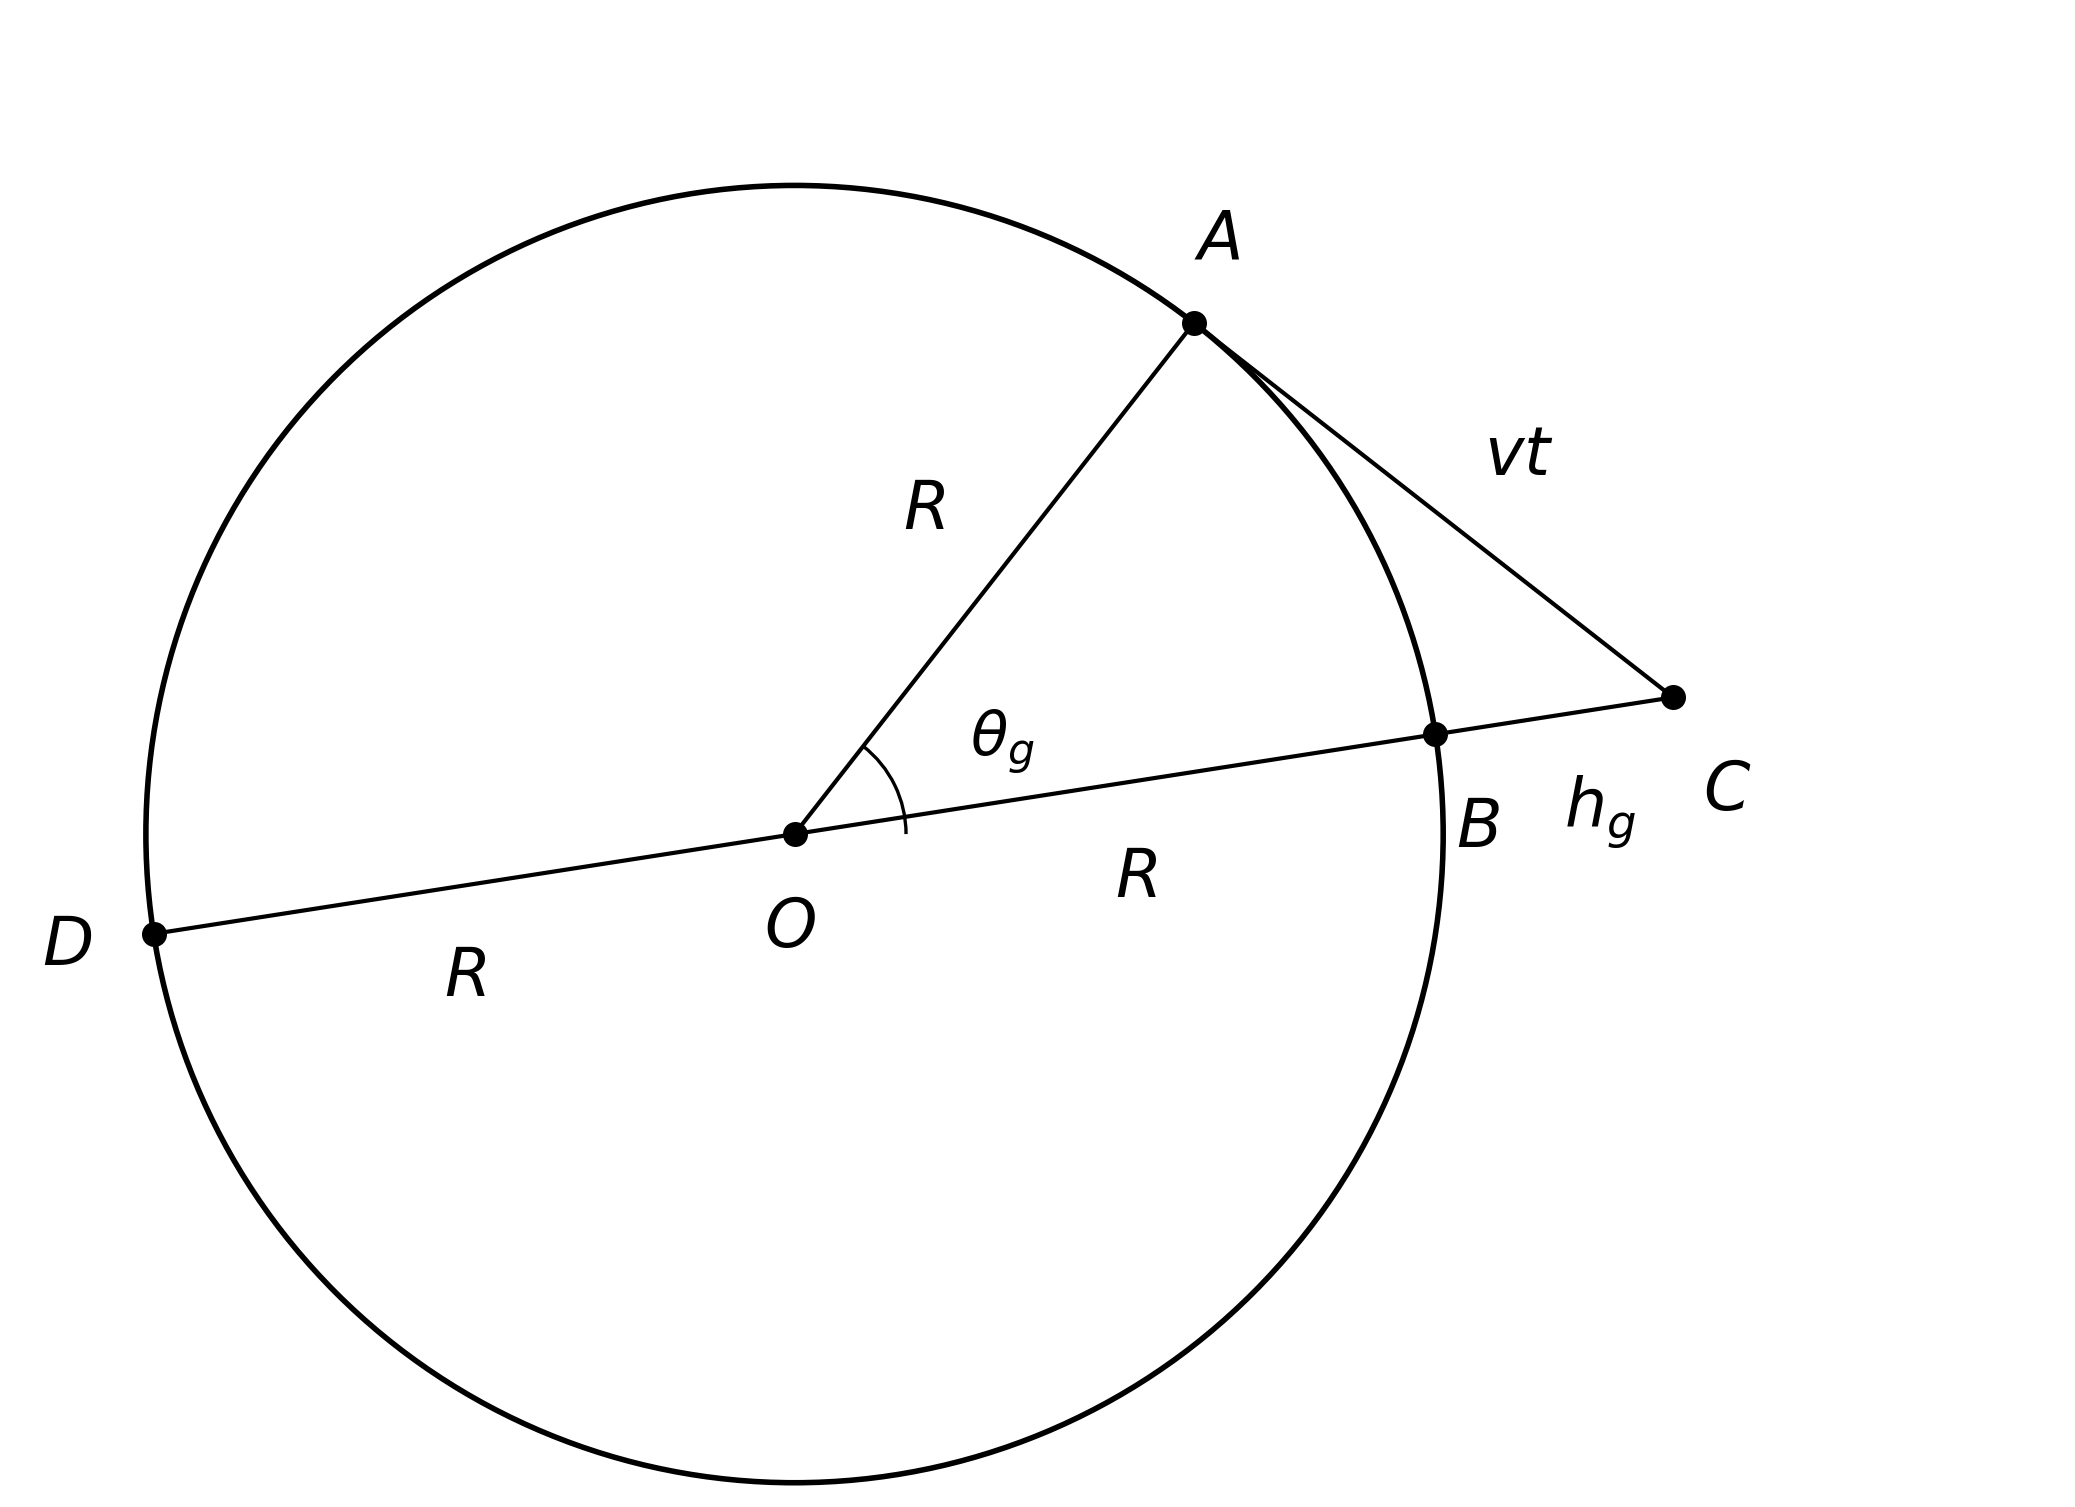
\includegraphics[width=0.7\textwidth]{centripetal_fig1.png}
\caption{Auxiliary tangent construction defining the geometrical deviation $h_g$.}
\label{fig:centripetal}
\end{figure}

\begin{proposition}[Tangent construction and power of the exterior point]
\label{prop:centripetal-power}
Let a circle have center $\pt{O}$ and radius $R$. At $\pt{A}$ on the circle, let $\seg{AC}$ be tangent with $\seglen{AC}=vt$. For every secant through the exterior point $\pt{C}$ meeting the circle at $\pt{X}$ and $\pt{Y}$,
\be
\seglen{CX}\,\seglen{CY}=(vt)^2.
\label{eq:family-power}
\ee
For the diametral secant through $\pt{C},\pt{B},\pt{O},\pt{D}$ of Figure~\ref{fig:centripetal}, with $h_g=\seglen{CB}$, this becomes
\be
h_g(2R+h_g)=(vt)^2.
\label{eqtheo1}
\ee
\end{proposition}

\begin{proof}
Because $\seg{CA}$ is tangent to the circle at $\pt{A}$, Proposition \ref{popsectan} gives, for any secant through $\pt{C}$ meeting the circle at $\pt{X}$ and $\pt{Y}$,
\be
\seglen{CX}\,\seglen{CY}=\seglen{CA}^{2}.
\ee
Using Equation~\eqref{eq:tangent-length}, the common value is $(vt)^2$, which proves Equation~\eqref{eq:family-power}. Choosing the secant through the center gives $\seglen{CB}=h_g$ and $\seglen{CD}=2R+h_g$, hence
\be
h_g(2R+h_g)=(vt)^2.
\ee
This is the desired diametral specialization of the secant-invariant power relation.
\end{proof}

The same identity can also be checked independently from the right triangle $\triangle \mathbf{OAC}$: because $\seg{OA}\perp\seg{AC}$,
\be
(R+h_g)^2=R^2+(vt)^2,
\label{pytha}
\ee
which factorizes into Equation~\eqref{eqtheo1}. The logical role of the power-of-a-point theorem is nevertheless broader than this check: Equation~\eqref{eq:family-power} states that the product is independent of the secant chosen through $\pt{C}$, whereas the Pythagorean calculation addresses only the special diametral secant. In the notation of \ref{app:power-point}, the exterior point therefore has the exact power
\be
\Pot_{\lambda}(\pt{C})=\seglen{CO}^{2}-R^2=\seglen{CA}^{2}=(vt)^2,
\label{eq:power-C}
\ee
where $\lambda$ denotes the circular orbit.

\section{Local Circular Kinematics and Centripetal Acceleration}\label{sec:local-kinematics}

The relation between normal deviation and normal acceleration is most clearly stated as a local property of the physical trajectory. Choose the time origin so that the particle is at the point $\pt{A}$ when $t=0$, and let $\mathbf{r}(t)$ denote its position vector. Assume that $\mathbf{r}$ is of class $C^3$ in a neighborhood of $t=0$. The Taylor expansion about $t=0$ is then
\be
\mathbf{r}(t)=\mathbf{r}_{\pt{A}}
+\left.\frac{\dd\mathbf{r}}{\dd t}\right|_{t=0}t
+\frac{1}{2}\left.\frac{\dd^2\mathbf{r}}{\dd t^2}\right|_{t=0}t^2
+O(t^3).
\label{eq:trajectory-taylor}
\ee
The instantaneous velocity and acceleration at $\pt{A}$ are therefore defined separately by
\begin{subequations}\label{eq:va-aa-definitions}
\begin{align}
\mathbf{v}_{\pt{A}}&\equiv\left.\frac{\dd\mathbf{r}}{\dd t}\right|_{t=0},
\label{eq:velocity-A}\\
\mathbf{a}_{\pt{A}}&\equiv\left.\frac{\dd^2\mathbf{r}}{\dd t^2}\right|_{t=0}.
\label{eq:acceleration-A}
\end{align}
\end{subequations}
Let $\mathbf{t}_{\pt{A}}=\mathbf{v}_{\pt{A}}/v$ be the unit tangent to the orbit at $\pt{A}$, and let $\mathbf{n}_{\pt{A}}$ be the inward unit normal, directed toward the center $\pt{O}$. These vectors are orthogonal, $\mathbf{t}_{\pt{A}}\!\cdot\!\mathbf{n}_{\pt{A}}=0$, and provide the local tangent--normal frame. The acceleration may consequently be decomposed as
\be
\mathbf{a}_{\pt{A}}=a_t\,\mathbf{t}_{\pt{A}}+a_n\,\mathbf{n}_{\pt{A}},
\label{eq:acc-decomposition}
\ee
where $a_t=\mathbf{t}_{\pt{A}}\!\cdot\!\mathbf{a}_{\pt{A}}$ is the tangential component and the inward normal component is
\be
 a_n\equiv\mathbf{n}_{\pt{A}}\!\cdot\!\mathbf{a}_{\pt{A}}.
\label{eq:normal-acc-component}
\ee
The zeroth- and first-order terms of Equation~\eqref{eq:trajectory-taylor} also have a direct geometrical meaning. If the inward interaction were removed at $\pt{A}$, the particle would preserve its instantaneous velocity and, after a time $t$, would reach the tangent point $\pt{C}$ of Figure~\ref{fig:centripetal}. The corresponding inertial tangent continuation has position
\be
\mathbf{r}^{\mathrm{tan}}_{\pt{C}}(t)=\mathbf{r}_{\pt{A}}+\mathbf{v}_{\pt{A}}t.
\label{eq:tangent-continuation}
\ee
The actual particle instead reaches a point $\pt{Q}$ on the circular orbit, with position $\mathbf{r}(t)$. The vector
\be
\Delta\mathbf{r}(t)\equiv\mathbf{r}(t)-\mathbf{r}^{\mathrm{tan}}_{\pt{C}}(t).
\label{eq:delta-r}
\ee
Therefore, it measures the departure of the physical trajectory from the inertial tangent continuation. In the local tangent--normal frame, $\Delta\mathbf{r}$ resolves into mutually orthogonal tangential and normal projections. Geometrically, these projections are the two legs of a right triangle whose hypotenuse is $\Delta\mathbf{r}$. Because $\mathbf{n}_{\pt{A}}$ is a unit vector perpendicular to $\mathbf{t}_{\pt{A}}$, taking the scalar product with $\mathbf{n}_{\pt{A}}$ removes the tangential projection and returns precisely the signed inward normal leg. We therefore define the local normal departure by
\be
h_c(t)\equiv\mathbf{n}_{\pt{A}}\!\cdot\!\Delta\mathbf{r}(t)
=\mathbf{n}_{\pt{A}}\!\cdot\!\left[\mathbf{r}(t)-\mathbf{r}_{\pt{A}}-\mathbf{v}_{\pt{A}}t\right].
\label{eq:normal-departure-definition}
\ee
Substituting the Taylor expansion and using Equation~\eqref{eq:normal-acc-component} gives
\be
h_c(t)=\frac{1}{2}a_n t^2+O(t^3).
\label{eq:normal-departure}
\ee
For uniform circular motion, the speed is constant. Hence
\be
\frac{\dd}{\dd t}\!\left(\mathbf{v}\!\cdot\!\mathbf{v}\right)
=2\,\mathbf{v}\!\cdot\!\mathbf{a}=0,
\label{eq:constant-speed-orthogonality}
\ee
so the acceleration has no tangential component. Since the circular trajectory bends toward its center, the remaining normal component is directed along $\mathbf{n}_{\pt{A}}$. In Newtonian terminology, this instantaneous inward component is the centripetal acceleration; the nontrivial magnitude relation is not assumed here but will be obtained from the geometrical construction. We therefore define
\be
 a_c\equiv a_n=\mathbf{n}_{\pt{A}}\!\cdot\!\mathbf{a}_{\pt{A}}>0.
\label{eq:centripetal-definition}
\ee
With this definition, Equation~\eqref{eq:normal-departure} becomes $h_c(t)=\tfrac12 a_c t^2+O(t^3)$, and therefore
\be
 a_c=\lim_{t\to0}\frac{2h_c(t)}{t^2}.
\label{eq:normal-acc-definition}
\ee
Equation~\eqref{eq:normal-acc-definition} is an instantaneous statement: it does not assume that the acceleration remains constant over a finite interval. Still, it identifies the normal acceleration as twice the quadratic coefficient that governs the separation between the physical trajectory and its tangent in the limit of arbitrarily short elapsed time. This is the modern local form of the geometrical limiting idea underlying Newtonian treatments of centripetal motion \cite{newton1729principia,erlichson1991motive}. The auxiliary geometrical deviation $h_g$ introduced in Equation~\eqref{eq:hg-definition} is distinct from $h_c$: $h_g$ is the radial gap from the tangent endpoint $\pt{C}$ to the circle measured along the ray through $\pt{C}$ and $\pt{O}$, whereas $h_c$ is the inward normal departure of the actual orbital point $\pt{Q}$ from the tangent continuation at $\pt{A}$. The two quantities are neither measured along the same direction nor based at the same point, so their relation must be established rather than assumed.

Uniform motion supplies the remaining kinematics. The distance traveled along the circle in time $t$ is $s=vt$, while $s=R\theta$. Introduce the dimensionless short-time parameter
\be
\tau\equiv\frac{vt}{R},
\label{eq:tau}
\ee
so that the physical angular position after time $t$ is $\theta=\tau$. By contrast, the auxiliary point $\pt{B}$ lies on the ray through $\pt{O}$ and $\pt{C}$, and the corresponding angle in Figure~\ref{fig:centripetal} is $\theta_g$. From the right triangle $\triangle \mathbf{OAC}$,
\be
\theta_g=\arctan\tau.
\label{eq:theta-g}
\ee
For any finite elapsed time, therefore, the auxiliary angle is $\theta_g=\arctan\tau$ whereas the physical orbital angle is $\theta=\tau$; the two are not equal in general. Replacing $\arctan\tau$ by $\tau$ is a small-angle approximation, justified only in the local regime $|\tau|=|vt|/R\ll1$, and it cannot be applied to an arbitrary finite $t$. Consequently, the auxiliary point $\pt{B}$ cannot in general be identified with the physical orbital point $\pt{Q}$. In the local limit,
\be
\arctan\tau=\tau-\frac{\tau^3}{3}+O(\tau^5),
\ee
so the angular distinction vanishes to first order. The crucial quadratic coefficient, however, can already be obtained directly from the exact power relation before any series expansion is used. Dividing Equation~\eqref{eqtheo1} by $t^2$ gives
\be
\left(2R+h_g\right)\frac{h_g}{t^2}=v^2.
\ee
Since $h_g\to0$ as $t\to0$,
\be
\lim_{t\to0}\frac{2h_g}{t^2}=\frac{v^2}{R}.
\label{eq:hg-limit}
\ee
Thus the power-of-a-point construction fixes the quadratic coefficient of the auxiliary deviation independently of the finite-time identification of $\pt{B}$ with the physical orbit.

The geometrical and physical deviations can now be compared explicitly. The geometrical deviation follows exactly from Equation~\eqref{eqtheo1}, or equivalently from Equation~\eqref{pytha}:
\be
h_g=\sqrt{R^2+v^2t^2}-R=R\left(\sqrt{1+\tau^2}-1\right),
\label{eq:hg-exact}
\ee
with short-time expansion
\be
h_g=\frac{v^2t^2}{2R}-\frac{v^4t^4}{8R^3}+O(t^6).
\label{eq:hg-expansion}
\ee
To write the physical normal deviation explicitly, choose Cartesian coordinates with $\pt{O}=(0,0)$, $\pt{A}=(R,0)$, and tangent line $x=R$. The actual orbital point after angular displacement $\theta=\tau$ is
\be
\pt{Q}=(R\cos\tau,R\sin\tau),
\label{eq:Q-coordinate}
\ee
and its distance from the tangent line measured along the inward normal is
\be
h_c=R-R\cos\tau=R(1-\cos\tau),
\label{eq:hc-exact}
\ee
which gives
\be
h_c=\frac{v^2t^2}{2R}-\frac{v^4t^4}{24R^3}+O(t^6).
\label{eq:hc-expansion}
\ee
Consequently,
\be
h_g-h_c=-\frac{v^4t^4}{12R^3}+O(t^6).
\label{eq:deviation-error}
\ee
The two deviations are not equal at finite time, but their difference is fourth order and therefore
\be
\lim_{t\to0}\frac{2(h_g-h_c)}{t^2}=0.
\ee
Combining this result with Equation~\eqref{eq:hg-limit} gives
\be
\lim_{t\to0}\frac{2h_c}{t^2}=\lim_{t\to0}\frac{2h_g}{t^2}=\frac{v^2}{R}.
\label{eq:local-equivalence}
\ee
Using Equation~\eqref{eq:normal-acc-definition}, one obtains
\be
a_c=\frac{v^2}{R},
\ee
with direction toward the center of the circle. In this ordering, the tangent--secant identity produces the quadratic coefficient of the auxiliary deviation, and Equation~\eqref{eq:deviation-error} justifies transferring that coefficient to the physical circular trajectory. A dimensionless measure of the finite-time discrepancy is obtained by normalizing with the physical deviation:
\be
\varepsilon(\tau)\equiv\frac{h_g-h_c}{h_c}=\frac{\sqrt{1+\tau^2}+\cos\tau-2}{1-\cos\tau}=-\frac{\tau^2}{6}+O(\tau^4).
\label{eq:relative-error}
\ee
This expression makes the short-time qualification quantitative without changing the role of the construction. For illustration, if a $1\%$ tolerance is adopted, $|\varepsilon(\tau)|=0.01$, the exact expression in Equation~\eqref{eq:relative-error} gives $\tau\simeq0.249876$, corresponding to an orbital angle of approximately $14.32^{\circ}$. The numerical threshold is not intrinsic to the derivation; it simply gives scale to the asymptotic statement. This distinction preserves the pedagogical content of the classical construction while separating two logically different statements. The equality $\seglen{CA}^{2}=\seglen{CX}\,\seglen{CY}$ is an exact invariant of Euclidean circle geometry. Its use in circular kinematics is local because the auxiliary intersection selected by a particular secant need not coincide with the finite-time orbital point. What survives in the short-time limit is the common second-order departure from the tangent, and that coefficient is precisely the centripetal acceleration.

\begin{remark}[Power associated with the tangent endpoint]
\label{rem:ac-power}
Equation~\eqref{eq:power-C} shows that the squared tangent displacement $\seglen{AC}^{2}=(vt)^2$ is the power of the exterior point $\pt{C}$ with respect to the circular orbit. Equation~\eqref{eq:family-power} adds the geometrically stronger statement that the same value is obtained from every secant through $\pt{C}$. The diametral secant is therefore not the definition of the correspondence but the most convenient member of a secant family for expressing the product in terms of $R$ and $h_g$.
\end{remark}

\section{Conclusion}

This work has examined a classical geometric route to centripetal acceleration and its correspondence to the tangent--secant relation in circle geometry. The historical attribution requires a clear distinction: the underlying segment-product relations are Euclidean, whereas Steiner's 1826 contribution \cite{steiner1826einige} introduced the power of a point as a unifying quantity. Newton's treatment of circular motion therefore belongs to a geometrical tradition that long predates the nineteenth-century terminology, even though the modern power-of-a-point language provides an efficient way to describe the structure of the construction. For the tangent endpoint $\pt{C}$, the exact geometrical statement is that $\Pot_{\lambda}(\pt{C})=\seglen{CA}^{2}=\seglen{CX}\,\seglen{CY}=(vt)^2$ for every secant through $\pt{C}$ meeting the circle at $\pt{X}$ and $\pt{Y}$. The diametral secant is the convenient member of this family for which the product becomes $h_g(2R+h_g)$. Thus, the Pythagorean factorization of the right triangle $\triangle \mathbf{OAC}$ verifies the selected configuration. At the same time, the power-of-a-point formulation identifies the common invariant shared by the complete secant family. The physical interpretation is local rather than finite-time exact. The auxiliary point $\pt{B}$ and the physical orbital point $\pt{Q}$ have angular positions $\theta_g=\arctan\tau$ and $\theta=\tau$, respectively, with $\tau=vt/R$. Correspondingly, $h_g$ is a radial gap measured along the ray through $\pt{O}$ and $\pt{C}$, whereas $h_c$ is the normal distance from $\pt{Q}$ to the tangent at $\pt{A}$. Their difference begins at fourth order, $h_g-h_c=-v^4t^4/(12R^3)+O(t^6)$, and their relative discrepancy satisfies $\varepsilon(\tau)=-\tau^2/6+O(\tau^4)$. A $1\%$ tolerance in $|\varepsilon|$ corresponds to $\tau\simeq0.249876$, or an orbital angle of approximately $14.32^{\circ}$. Nevertheless, the exact power relation fixes the common quadratic coefficient, and the local trajectory expansion then gives the familiar centripetal acceleration $a_c=v^2/R$. The distinction between exact Euclidean identity and local physical interpretation is therefore the central qualification established by the construction.

The pedagogical value of the argument lies in demonstrating the relationship among inertial motion, curvature, and classical circle geometry before introducing more advanced analytical machinery. The historical and pedagogical literature reviewed in Section 2 shows that this objective has motivated tangent-displacement, trigonometric, velocity-space, and historically reconstructed derivations. The present treatment retains the classical proofs in Appendix~\ref{app:power-point}, while making explicit the distinct roles of Euclidean geometry, Steiner's later invariant language, and local circular kinematics. No classroom validation or comparative educational study is claimed here.

\bibliographystyle{unsrturl}
\bibliography{centripetal}



\clearpage
\appendix
\setcounter{subsection}{0}
\renewcommand{\thesubsection}{A.\arabic{subsection}}
\setcounter{figure}{0}
\renewcommand{\thefigure}{A.\arabic{figure}}
\renewcommand{\theproposition}{A.\arabic{proposition}}
\section{Power of a Point in Classical Circle Geometry}\label{app:power-point}

\subsection{Historical clarification and notation}

The segment-product relations used in this article belong to classical Euclidean circle geometry. In particular, the intersecting-chords and tangent--secant configurations appear in Euclid's \textit{Elements}, Book III, Propositions 35 and 36 \cite{euclid1956elements}. Steiner's contribution in 1826 \cite{steiner1826einige} was of a different kind: he introduced the notion of power as a quantity associated with a point and a circle, thereby providing a unified algebraic interpretation of these classical configurations. Newton's geometrical mechanics therefore predates Steiner and was developed within a mathematical tradition in which the underlying Euclidean results were already available. For completeness, and to keep the subsequent correspondence self-contained, we briefly recall the classical proofs of the segment-product relations used in Section~\ref{sec:exact-geometry}. These results are standard; their inclusion in this appendix is intended to fix the notation and make explicit the geometrical structure required by the physical argument. Throughout this section, point labels are set in bold upright type, and $\seglen{XY}$ denotes the ordinary positive length of the segment joining $\pt{X}$ and $\pt{Y}$. When directed segments are introduced later, $\dseg{XY}$ denotes the corresponding signed segment along an oriented secant. The three Euclidean configurations considered below are not independent results but different manifestations of the same segment-product structure. We first recall them in their usual positive-length form and then collect them into the signed power-of-a-point formulation.

\subsection{Classical segment-product configurations}

Figure~\ref{steinerpop} summarizes the three standard geometrical configurations. The first involves two chords intersecting inside the circle; the second involves two secants drawn from an exterior point; the third is the tangent--secant limiting case. The proofs are included only to make the later mechanical correspondence explicit and self-contained.

\begin{figure}[ht]
    \centering
    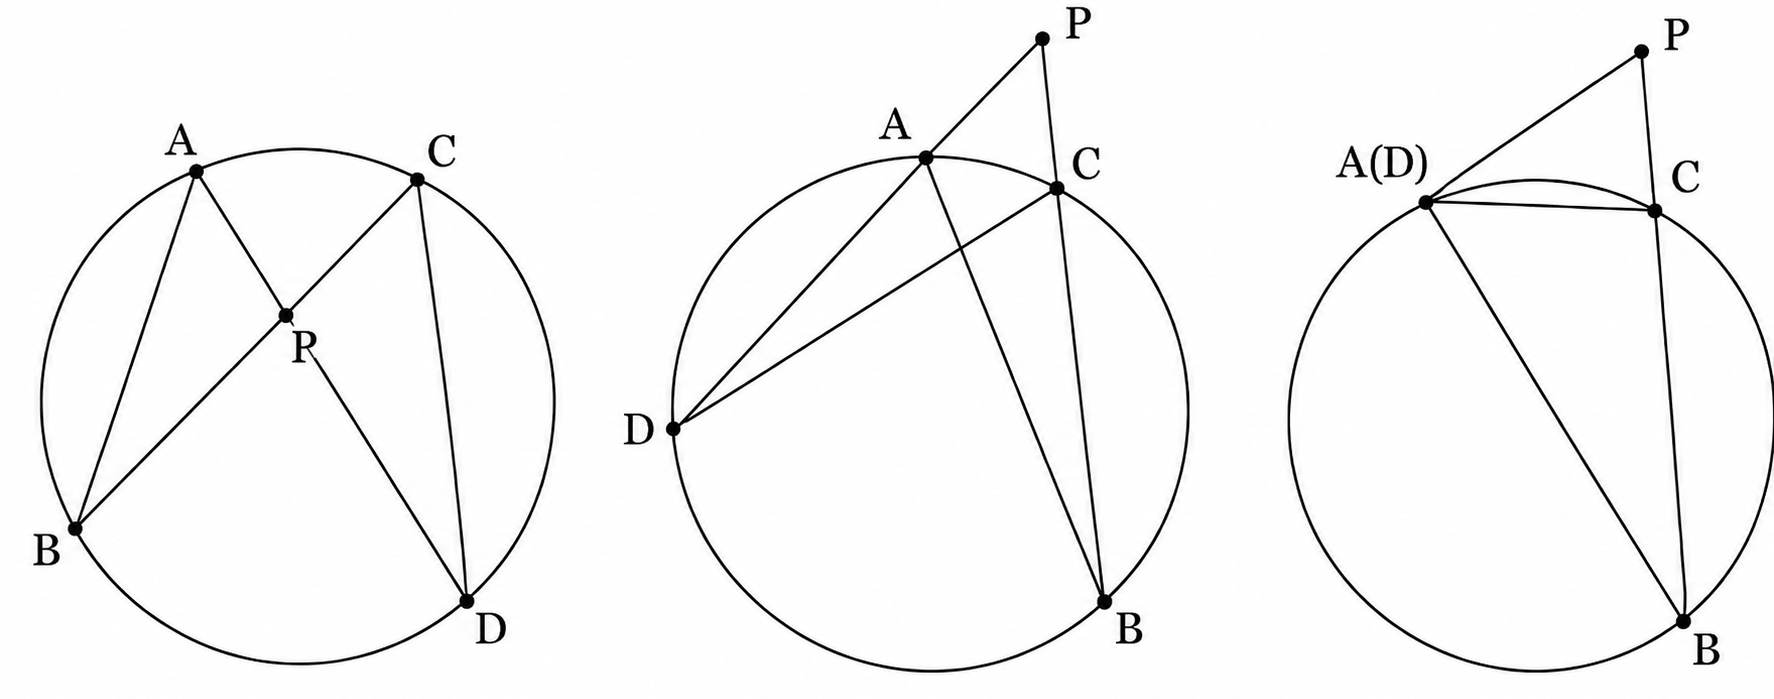
\includegraphics[width=0.82\textwidth]{steinerpop.png}
    \caption{Classical intersecting-chords, exterior-secant, and tangent--secant configurations.}
    \label{steinerpop}
\end{figure}

\begin{proposition}[Intersecting chords]
\label{pop2chords}
Let $\seg{AD}$ and $\seg{CB}$ be two chords of a circle intersecting at an interior point $\pt{P}$, as shown in the first panel of Figure~\ref{steinerpop}. Then
\be
\seglen{AP}\,\seglen{DP}=\seglen{BP}\,\seglen{CP}.
\ee
\end{proposition}

\begin{proof}
Consider $\triangle \mathbf{ABP}$ and $\triangle \mathbf{CDP}$. The angles $\angle \mathbf{ABP}$ and $\angle \mathbf{CDP}$ subtend the same chord $\seg{AC}$, while $\angle \mathbf{APB}$ and $\angle \mathbf{CPD}$ are vertically opposite. Hence $\triangle \mathbf{ABP}\sim\triangle \mathbf{CDP}$, so
\be
\frac{\seglen{AP}}{\seglen{CP}}=\frac{\seglen{BP}}{\seglen{DP}},
\ee
which gives $\seglen{AP}\,\seglen{DP}=\seglen{BP}\,\seglen{CP}$.
\end{proof}

The intersecting-chords identity already exhibits the essential invariant structure. Once the point of intersection is fixed, the product of the two directed distances along one line is equal to the corresponding product along the other. For an interior point, however, the use of ordinary positive lengths hides the sign that later appears naturally in the definition of power.

\begin{proposition}[Two secants from an exterior point]
\label{pop2sec}
Let $\pt{P}$ be a point outside a circle. Let two secants from $\pt{P}$ intersect the circle at $\pt{A},\pt{D}$ and $\pt{C},\pt{B}$, respectively, with $\pt{A}$ and $\pt{C}$ the nearest intersection points to $\pt{P}$, as shown in the second panel of Figure~\ref{steinerpop}. Then
\be
\seglen{PA}\,\seglen{PD}=\seglen{PC}\,\seglen{PB}.
\ee
\end{proposition}

\begin{proof}
Consider $\triangle \mathbf{PAB}$ and $\triangle \mathbf{PCD}$. They share the angle at $\pt{P}$, and the remaining relevant angles are equal because the corresponding inscribed angles subtend the same chord $\seg{DB}$. Therefore $\triangle \mathbf{PAB}\sim\triangle \mathbf{PCD}$, which gives
\be
\frac{\seglen{PA}}{\seglen{PC}}=\frac{\seglen{PB}}{\seglen{PD}},
\ee
and hence $\seglen{PA}\,\seglen{PD}=\seglen{PC}\,\seglen{PB}$.
\end{proof}

For an exterior point, both factors in each product are positive when ordinary lengths are used. This is the form most directly connected with the construction employed in Section~\ref{sec:exact-geometry}.

\begin{proposition}[Tangent--secant form]
\label{popsectan}
Let $\pt{P}$ be a point outside a circle. Let $\seg{PA}$ be tangent to the circle at $\pt{A}$, and let a secant from $\pt{P}$ intersect the circle first at $\pt{C}$ and then at $\pt{B}$, as shown in the third panel of Figure~\ref{steinerpop}. Then
\be
\seglen{PC}\,\seglen{PB}=\seglen{PA}^{2}.
\ee
\end{proposition}

\begin{proof}
Consider $\triangle \mathbf{PAC}$ and $\triangle \mathbf{PBA}$. The angle at $\pt{P}$ is common. By the tangent--chord theorem, the angle between the tangent $\seg{PA}$ and chord $\seg{AC}$ equals the inscribed angle subtended by the same chord, so the triangles are similar. Therefore
\be
\frac{\seglen{PA}}{\seglen{PB}}=\frac{\seglen{PC}}{\seglen{PA}},
\ee
which yields $\seglen{PA}^{2}=\seglen{PC}\,\seglen{PB}$.
\end{proof}

The tangent--secant form is the configuration required later. Its relevance is not merely that one particular secant reproduces the squared tangent length, but that every secant through the same exterior point yields the same segment product. This secant invariance is the geometrical content that becomes especially transparent in the language of power of a point.

\subsection{Signed power of a point}

The three configurations above can be unified by introducing the signed power of a point. Let $\lambda$ be a circle with center $\pt{O}$ and radius $R$. The power of a point $\pt{P}$ with respect to $\lambda$ is
\be
\Pot_{\lambda}(\pt{P})=\seglen{PO}^{2}-R^2.
\label{eq:power-definition}
\ee
Therefore,
\be
\begin{cases}
\Pot_{\lambda}(\pt{P})>0, & \text{if } \pt{P} \text{ lies outside the circle }(\seglen{PO}>R),\\[4pt]
\Pot_{\lambda}(\pt{P})=0, & \text{if } \pt{P} \text{ lies on the circle }(\seglen{PO}=R),\\[4pt]
\Pot_{\lambda}(\pt{P})<0, & \text{if } \pt{P} \text{ lies inside the circle }(\seglen{PO}<R).
\end{cases}
\ee
For an exterior point, ordinary positive lengths give
\be
\Pot_{\lambda}(\pt{P})=\seglen{PA}\,\seglen{PD}=\seglen{PC}\,\seglen{PB},
\ee
and, for a tangent,
\be
\Pot_{\lambda}(\pt{P})=\seglen{PT}^{2}.
\ee
For an interior point, the positive-length chord relation remains positive while the signed power is negative:
\be
\Pot_{\lambda}(\pt{P})=-\seglen{PA}\,\seglen{PD}=-\seglen{PB}\,\seglen{PC}.
\ee
The sign difference is purely geometrical: for an interior point, the two intersections on any secant lie on opposite sides of $\pt{P}$. Directed segments therefore provide a natural way to absorb the sign into the product itself. Orient each secant line and interpret $\dseg{PX}$ as the signed coordinate difference from $\pt{P}$ to $\pt{X}$ along that oriented line. Then the relation can be written uniformly as
\be
\dseg{PA}\,\dseg{PD}=\dseg{PB}\,\dseg{PC}=\Pot_{\lambda}(\pt{P}).
\label{eq:directed-power}
\ee
Figure~\ref{steinerpop2} illustrates three complementary interpretations using ordinary positive lengths. In panel (a), $\pt{P}$ lies outside the circle and $\seg{PT}$ is tangent at $\pt{T}$, so the power is positive and equals $\seglen{PT}^{2}$. In panel (b), $\pt{P}$ lies inside the circle and $\seg{PS}$ is perpendicular to $\seg{PO}$ with $\pt{S}$ on the circle; the right triangle $\triangle \mathbf{OPS}$ gives $\seglen{PS}^{2}=R^2-\seglen{PO}^{2}=-\Pot_{\lambda}(\pt{P})$. In panel (c), $\pt{P}$ lies outside the circle and a secant intersects it at $\pt{S}_1$ and $\pt{S}_2$, giving $\seglen{PS_1}\,\seglen{PS_2}=\Pot_{\lambda}(\pt{P})$.

\begin{figure}[ht]
\centering
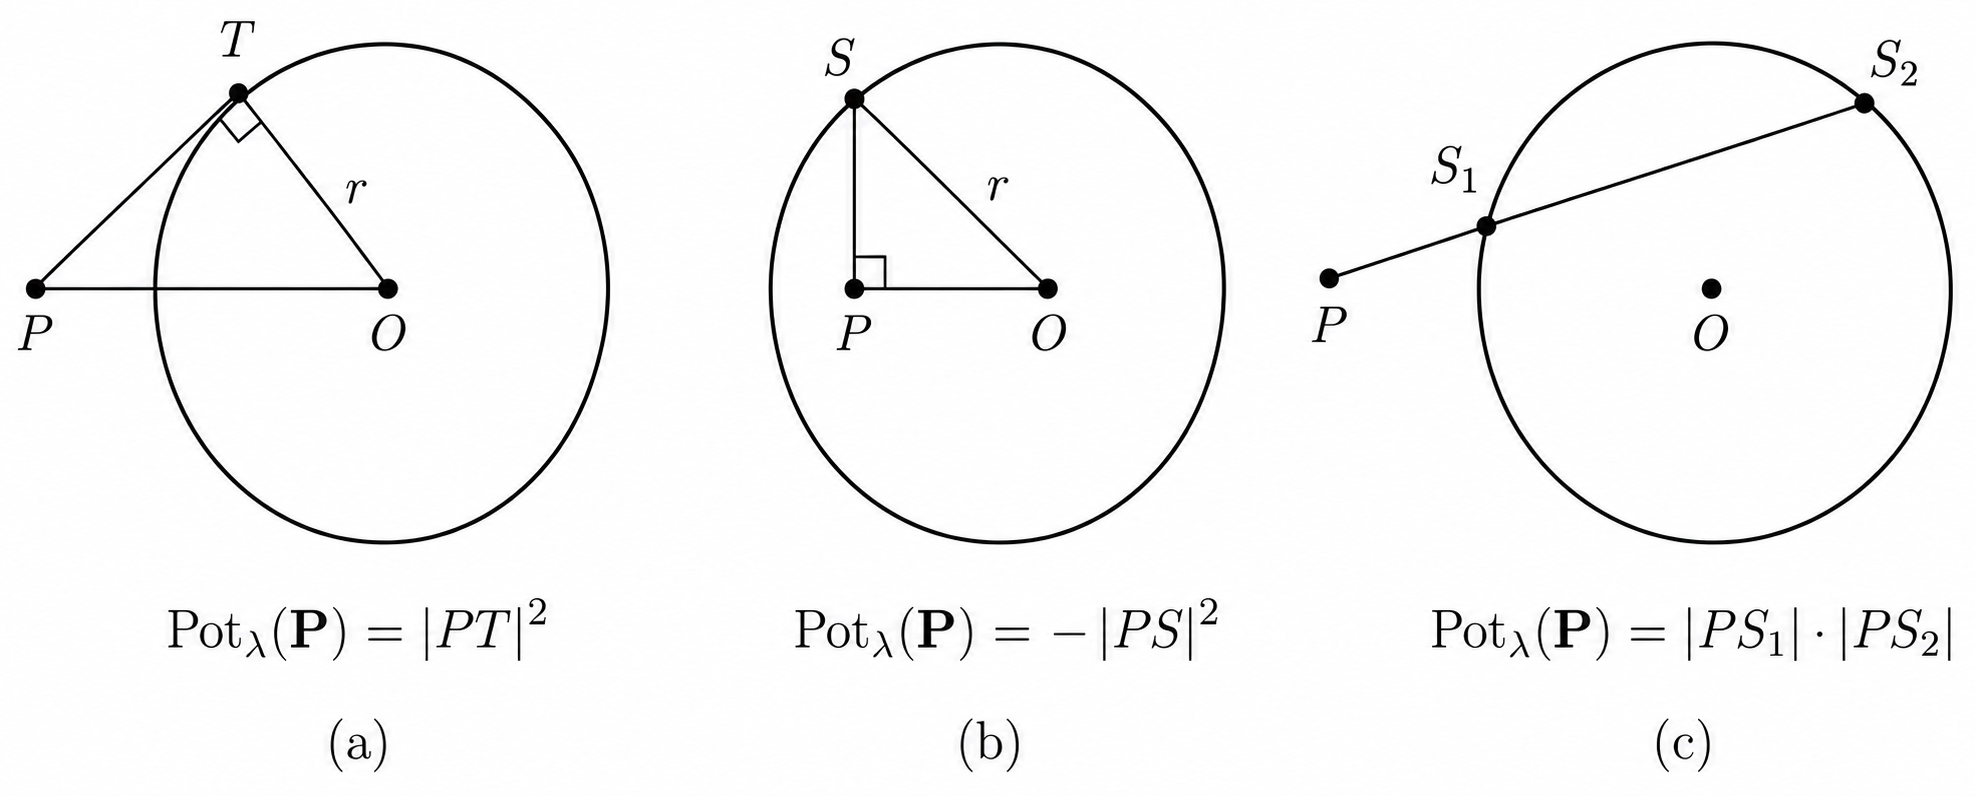
\includegraphics[scale=0.2]{steinerpop2.png}
\caption{Signed power of a point with respect to a circle of center $\pt{O}$ and radius $R$. (a) For an exterior point, $\Pot_{\lambda}(\pt{P})=\seglen{PT}^{2}>0$. (b) For an interior point, $\Pot_{\lambda}(\pt{P})<0$ and $\seglen{PS}^{2}=-\Pot_{\lambda}(\pt{P})$. (c) For an exterior secant, $\Pot_{\lambda}(\pt{P})=\seglen{PS_1}\,\seglen{PS_2}>0$.}
\label{steinerpop2}
\end{figure}

The main point for the mechanical application is now explicit. The tangent length and every secant product through a fixed exterior point represent the same invariant quantity. Section~\ref{sec:exact-geometry} applies precisely this exterior-point form to the tangent endpoint generated by inertial motion.

\end{document}
